\documentclass[12pt]{scrartcl}
\usepackage[pretty]{mystd}
\title{Classification des surfaces compactes, connexes et orientables par la théorie de Morse}
\author{Amar Ahmane\\ Sous la direction d'Anne Vaugon}
\date{ENS Ker Lann, 2023/2024}

\tikzset{
  state/.style={circle,draw,minimum size=6ex},
  arrow/.style={-latex, shorten >=1ex, shorten <=1ex}}

\begin{document}
\maketitle
\tableofcontents

{\small
\setlength{\parindent}{0em}
\setlength{\parskip}{1em}
}

\newpage

%%%%%%%%%%%%%%%%
% INTRODUCTION %
%%%%%%%%%%%%%%%%

% TODO : dans cette section, inclure les références bibliograpgiques 
% lorsqu'il y a mention de livres/articles utilisés.
% Réécrire la partie du rapport qui dit que je vais prouver des trucs 
% que je n'ai pas prouvé, et les démontrer. 

\section{Introduction}
La théorie de Morse, du mathématicien américain 
Marston Morse (1892 - 1972), part de l'idée que 
l'étude de fonctions très bien choisies sur une 
variété permet d'en étudier la topologie. 
C'est un ensemble de résultats de topologie et 
de géométrie différentielles qui, de manière 
plus précise, permet de relier l'étude de la 
topologie de l'espace sur lequel on définit 
certaines fonctions différentiables à l'étude 
des points critiques de ces fonctions différentiables.


Le thème de mon stage a été la théorie de Morse. 
Celui-ci a commencé le 27 mai 2024 et a duré 6 semaines.
Il a pris place au sein du laboratoire de mathématiques 
d'Orsay,  dans l'équipe de topologie et dynamique.
L'objectif était de me familiariser avec des notions et 
des éléments de la théorie de Morse pour pouvoir les 
appliquer dans la démonstration de la classification des 
surfaces compactes, connexes, orientables et sans bord.

Ce travail a commencé par l'étude de notions de base de 
topologie différentielle, notamment en étudiant le cours 
du même nom de Patrick Massot, ce qui a permis ensuite 
l'étude de différents livres portant essentiellement sur 
la théorie de Morse, tels que le célèbre \textit{Morse Theory} 
de J. Milnor ou le livre \textit{Théorie de Morse et Homologie de Floer} 
de Michèle Audin et Mihai Damian. Le présent document 
constitue le rapport du stage en question, où je résume 
ce que j'ai pu apprendre et en développant une preuve de 
la classification des surfaces compactes, connexes, orientables 
et sans bord.


Le rapport est découpé en trois parties.  Dans une première 
partie, que je nomme "Préliminaires", je présente quelques 
notions de base de topologie différentielle essentielles 
dans le travail qui suivra, où je montrerai notamment quelques 
résultats, comme le fait que toute variété compacte peut être 
plongée dans un espace affine, ou qu'un champ de vecteurs lisse 
qui s'annule en dehors d'un compact engendre un unique groupe 
à un paramètre de difféomorphes (un résultat qui sera utilisé 
dans la plupart des théorèmes de la section sur les fonctions 
de Morse sur les surfaces). La deuxième partie contient l'essentiel 
des résultats que j'ai vus pendant ce stage, commencera bien sûr 
par des définitions : qu'est-ce que c'est qu'une fonction de Morse ? 
Elle contiendra une preuve du lemme de Morse, une justification de 
l'existence de telles fonctions sur une variété et trois gros théorèmes 
qui concerneront les valeurs régulières d'une fonction de Morse sur une 
surface ainsi que le changement de topologie lors du passage d'une valeur 
critique.  Cette partie contiendra aussi quelques résultats concernant
les modifications de fonctions de Morse, essentielles pour la preuve de 
la classification. La dernière partie se sert enfin des résultats prouvés 
dans les sections précédentes pour établir la classification.


Je remercie évidemment ma tutrice de stage pour m'avoir accueilli, et 
de m'avoir invité à assister à certaines conférences à l'Institut Henri 
Poincaré notamment.



\newpage

%%%%%%%%%%%%%%%%%
% PRÉLIMINAIRES %
%%%%%%%%%%%%%%%%%

\section{Préliminaires}
Cette section permet d'introduire quelques notions et 
de définir des surfaces qui seront utilisées plus tard 
pour énoncer et démontrer la classification des surfaces.
On fera également des rappels de topologie différentielle. 

\subsection{Variétés et sous-variétés}
On rappelle qu'une variété topologique de dimension $n$ est 
un espace topologique séparé et $\sigma$-compact dont tous 
les points admettent un voisinage ouvert homéomorphe à un ouvert de $\R^n$.

On rappelle également que si $X$ est une variété topologique 
de dimension $n$, une carte est un homéomorphisme d'un ouvert 
de $X$ vers un ouvert de $\R^n$. Un atlas sur $X$ est une famille 
$\lbrace \varphi_i:U_i\to V_i\rbrace$ de cartes sur $X$ telle que 
$\bigcup_iU_i=X$.  Dans un atlas $\mathcal A=\lbrace \varphi_i:U_i\to V_i\rbrace$, 
on appelle changement de carte les applications 
$\varphi_{ij}=\varphi_j\circ\varphi_i^{-1}:\varphi_i(U_i\cap U_j)\to \varphi_j(U_i\cap U_j)$.
Un atlas est lisse lorsque tous ses changements de cartes sont lisses. 
Deux atlas lisses sont équivalents si leur réunion est encore un atlas lisse.

\begin{defi}
    Une variété différentielle (de classe $\mathcal C^\infty$) est la donnée 
    d'une paire $(X,\Sigma)$ où $X$ est une variété topologique et où $\Sigma$ 
    est une classe d'équivalence d'atlas lisses sur $X$.
\end{defi}

On parle ainsi de \textit{structure} de variété différentielle. 
Comme pour les groupes ou autre structures algébriques, on pourra 
parler d'une "variété différentielle $X$" au lieu de "variété différentielle $(X,\Sigma)$", 
la structure étant la plupart du temps sous-entendue dans les notations.
Dans toute la suite, le mot "variété" désignera une variété différentielle 
de classe $\mathcal C^\infty$.  Une surface sera alors une variété de 
dimension $2$. Des exemples de surfaces (et donc de variétés) sont la 
sphère $\mathbb S^2$, le tore $\mathbb T^2$, le ruban de Möbius, la bouteille de Klein... 

\begin{center}
    \begin{tikzpicture}[scale=.4]
    % Boule
    \shade[ball color=gray!90,opacity = 0.2] (0,0) circle (4cm);
	\draw[thick] (0,0) circle (4cm);
	\draw[thick] (-4,0) arc (180:360:4 and 0.6);
	\draw[thick,dashed] (4,0) arc (0:180:4 and 0.6);
    %% Ouvert Ui
    \node (p1) at (-2.5, -0.4) {};
    \node (p2) at (-0.5, 2.0) {};
    \node (p3) at (0.4, 0.1) {};
    \path[fill,AccColor1!50,opacity=0.5]plot [smooth cycle,tension=1] coordinates {(p1) (p2) (p3)};
    \node at (-1.8, 2.0) {$U_i$};
    % Ouvert Uj
    \node (q1) at (-0.5,0) {};
    \node (q2) at (2.0,-1) {};
    \node (q3) at (2.0, 0.5) {};
    \node (q4) at (-0.5, 1.0) {};
    \path[fill,AccColor2!50,opacity=0.5]plot [smooth cycle,tension=1] coordinates {(q1) (q2) (q3)(q4)};
    \path[thick,draw,black]plot [smooth cycle,tension=1] coordinates {(q1) (q2) (q3)(q4)};
    \path[thick,draw,black]plot [smooth cycle,tension=1] coordinates {(p1) (p2) (p3)}; 
	\node at (2,1.1) {$U_j$};

    % Ouvert d'arrivée i
    \node (p1) at (8, 2) {};
    \node (p2) at (12.5, 5.0) {};
    \node (p3) at (12.4, 2.1) {};
    \path[fill,AccColor1!30]plot [smooth cycle,tension=1] coordinates {(p1) (p2) (p3)};
    \path[thick,draw,black]plot [smooth cycle,tension=1] coordinates {(p1) (p2) (p3)}; 
	\node at (10.5,2.8) {$\varphi_i(U_i)$};
    
    % Ouvert d'arrivée j
    \node (q1) at (8.0,-5) {};
    \node (q2) at (12.5,-5.2) {};
    \node (q3) at (12.5, -2.3) {};
    \node (q4) at (8.3, -2.3) {};
    \path[fill,AccColor2!30]plot [smooth cycle,tension=1] coordinates {(q1) (q2) (q3)(q4)};
    \path[thick, draw, black]plot [smooth cycle,tension=1] coordinates {(q1) (q2) (q3)(q4)};
    \node at (10.5,-3.7) {$\varphi_j(U_j)$};

    % Flèche changement de carte
	\node at (16.2,3) {$\varphi_i (U_i \cap U_j)$};
	\draw [very thick, arrow] (16.2,-3) to (16.2,2) ;
	\node at (16.2,-4.2) {$\varphi_j (U_i \cap U_j)$};
	\node at (15.5,-0.5) [left] {$\varphi_{ij}$};

    % Flèches cartes
	\draw [very thick,arrow,bend angle=45,bend left]  (-0.2,1.2)  to (8.4,3) ;
	\node at (5,4.7) {$\varphi_i$};
	\draw [very thick,arrow,bend angle=45,bend right]  (0.5,0)  to (7.5,-5) ;
	\node at (5,-4.2) {$\varphi_j$};
\end{tikzpicture}\\
    \vspace{1em}
    \textsc{Figure 1} – \textit{Changements de cartes}
\end{center}

\begin{defi}
    Une partie $Y$ d'une variété $X$ de dimension $n$ est une sous-variété 
    de codimension $k\leq n$ si tout point de $Y$ est contenu dans le domaine 
    d'une carte $\varphi:U\hookrightarrow\R^n$ vérifiant 
    \[
        \varphi(Y\cap U)=\varphi(U)\times(\R^{n-k}\times\lbrace 0\rbrace)
    \]
\end{defi}

On voit très facilement qu'il est possible de munir une sous-variété $Y$ 
d'une structure de variété, simplement par restriction des cartes sur $X$.

\begin{remark}
    On retrouve bien la définition de sous-variété de $\R^n$ vue dans le cours 
    de calcul différentiel de L3, en choisissant le bon atlas lisse sur $\R^n$.
\end{remark}

\subsection{Applications différentiables sur des variétés}

\begin{defi}
    Soit $f:M\to N$ une application entre deux variétés de dimensions $n$ et 
    $p$ respectivement. Soit $x\in M$. On dit que $f$ est différentiable 
    (resp. lisse) en $x$ s'il existe des cartes $\varphi:U\to \R^n$ et $\psi:V\to\R^p$
    autour de $x$ et $f(x)$ respectivement telles que $\psi\circ f\circ\varphi^{-1}$ 
    est différentiable (resp. $\mathcal C^\infty$) en $\varphi(x)$.
\end{defi}

En particulier, une fonction $f:S\to \R$ partant d'une surface $S$ est lisse si 
pour toute carte $\varphi:U\to\R^2$, $f\circ\varphi^{-1}$ est lisse. Sauf mention 
du contraire, toutes les applications entre variétés seront supposées lisses dans 
la suite du document.

\begin{center}
    \input{figures/tikz/diff-map.tex}
    \textsc{Figure 2} – \textit{Application différentiable entre variétés}
\end{center}

Nous allons à présent définir les notions d'immersion, submersion, plongement et de 
difféomorphisme entre deux variétés. 

\begin{defi}
    Une application $f:X\to Y$ différentiable entre deux variétés de dimensions $n$ 
    et $p$ respectivement est appelée 
    \begin{enumerate}[(i)]
        \item une immersion si son rang vaut partout $n$;
        \item une submersion si son rang vaut partout $p$;
        \item un difféomorphisme local si son rang vaut partout $n$ et $p$.
    \end{enumerate}
    Un difféomorphisme entre deux variétés est une application lisse bijective dont 
    la réciproque est aussi lisse.  Un plongement d'une variété $N$ dans une variété 
    $M$ est une immersion $f$ qui est un homéomorphisme sur son image. 
\end{defi}

Ainsi, lorsqu'il existe un difféomorphisme entre deux variétés, on dira qu'elles sont 
difféomorphisme.

Le but, comme énoncé en introduction, est de classifier, à homéomorphisme près, les 
surfaces connexes, compactes et orientables (la notion d'orientable sera définie un 
peu plus bas). Par ailleurs, dans toute la suite, le mot "surface" désignera une surface 
connexe, compacte et orientable.

\begin{defi}
    Soient $f_0,f_1:M\to M$ des difféomorphismes où $M$ est une variété.
    Les applications $f_i$ sont dites homotopes s'il existe une application lisse 
    (une homotopie lisse) $F:[0,1]\times M\to M$ telle que 
    \begin{enumerate}[(i)]
        \item $\forall x\in M, F(0,x)=f_1(x)$;
        \item $\forall x\in M, F(1,x)=f_2(x)$;
        \item Pour tout $t\in[0,1]$, l'application $F(t,\cdot)$ est un difféomorphisme.
    \end{enumerate}
\end{defi}

\subsection{Fibré tangent, champ de vecteurs et groupe à paramètre}
\begin{defi}
    On considère $M$ une variété et $x\in M$. On note $C_xM$ l'ensemble des courbes 
    lisses passant par $x$ en $0$.
    On dit que deux éléments $\gamma_0$ et $\gamma_1$ de $C_xM$ ont même vitesse en 
    $0$ s'il existe une carte $\varphi:V\to\R^n$ telle que $V$ contient $x$ et 
    $\varphi\circ\gamma_0$ et $\varphi\circ\gamma_1$ ont même dérivée en $0$.
    Ainsi, l'espace tangent $T_xM$ de $M$ en $x$ est le quotient de $C_xM$ par la 
    relation d'équivalence "avoir la même vitesse en $0$". 
    On définit l'ensemble $TM$, réunion disjointe des $\lbrace p\rbrace\times T_pM$ 
    pour $p\in M$, que l'on appelle fibré tangent.
\end{defi}

\begin{remarks}
    \begin{itemize}
        \item Les espaces tangents $T_xM$ peuvent être munis d'une structure d'espace 
        vectoriel, leur dimension étant celle de la variété $M$ ;
        \item Le fibré tangent $TM$ peut-être muni d'une structure de variété, sa 
        dimension est égale à deux fois celle de $M$.
    \end{itemize}
\end{remarks}

\begin{center}
    \begin{tikzpicture}[x=0.75pt, y=0.75pt, yscale=-1, scale=.75]
    height of 300
  
    % The manifold
    \draw[thick] (112.04,66.62) node[above right, font=\scriptsize]{$M$};
    \draw[thick] (100,108) .. controls (140,78) and (188,143) 
                    .. (196,182) ;
    \draw[thick] (196.2,181.8) .. controls (211.8,159.6) and (265.71,101.03) 
                        .. (318.8,111.8) ;
    \draw[thick] (318.8,111.8) .. controls (323.67,112.42) and (330.33,115.42) 
                        .. (335,118) ;
    \draw[dotted] (219.48,53.8) .. controls (230.71,56.06) and (244.01,58.07) 
                                .. (259,63.39) ;
    \draw[thick] (259,63.39) .. controls (288.81,75.27) and (332.14,114.93) 
                      .. (335,118) ;
    \draw[thick] (100,108) .. controls (113.56,84.56) and (160.04,48.06) 
                    .. (219.48,53.8) ;
  
    % The tangent space at x
    \draw[thick] (238.68,46.2) -- (294.01,93.72) 
                        -- (224.01,122.72) 
                        -- (168.68,75.2) 
                        -- cycle ;
    \fill[AccColor2!40,opacity=.5] (238.68,46.2) -- (294.01,93.72) 
                        -- (224.01,122.72) 
                        -- (168.68,75.2) 
                        -- cycle ;                        
    \draw (173.51,76.9) node[below right, 
                             font=\scriptsize, 
                             rotate=-337.86,
                             xslant=-0.54]{$T_{x} M$};

    % A point x in the manifold
    \filldraw (232.9,84.2) circle (1pt)
    node[below right, font=\scriptsize]{$x$};
  \end{tikzpicture}\\
    \vspace{1em}
    \textsc{Figure 3} – \textit{Espace tangent en $x$}
\end{center}

Lorsque $M$ et $N$ sont des variétés et que $f:M\to N$ est une application lisse, 
cette dernière induit une application $C_xf:C_xM\to C_{f(x)}N$ pour $x\in M$ qui 
envoie $\gamma$ sur $f\circ \gamma$.

\begin{defi}
    L'application tangente à $f:M\to N$ en un point $x$ est l'application 
    $T_xf:T_xM\to T_{f(x)}N$ induite par $C_xf$.
    On définit $Tf:TM\to TN$ par $Tf(x,v)=(f(x),T_xf(v))$, aussi notée $\dd f$ ou $f_*$.
\end{defi}

À présent, on définit la notion de champ de vecteurs sur une variété.

\begin{defi}
    Un champ de vecteurs sur une variété $M$ est une application $X:M\to TM$
    telle que pour tout $x\in M$, $X(x)\in\lbrace x\rbrace\times T_xM$.
\end{defi}
Comme mentionné dans une précédente remarque, $TM$ est une variété, on peut alors 
parler de champ de vecteurs \textit{lisse}.

\begin{defi}
    Un groupe de paramètre de difféomorphismes d'une variété $M$ est une application 
    $\varphi:\R\times M\to M$ telle que 
    \begin{enumerate}[(i)]
        \item pour tout $t\in\R$, l'application $\varphi_t=\varphi(t,\cdot):M\to M$ est 
        un difféomorphisme ;
        \item pour tous $s$ et $t$, on a $\varphi_{s+t}=\varphi_t\circ\varphi_s$, en 
        particulier $\varphi_0=\id_M$.
    \end{enumerate}
\end{defi}

Étant donné $\varphi$ un groupe à paramètre de difféomorphismes, on définit un champ de 
vecteurs $X$ comme suit : au point $x\in M$, on pose 

\[
    X(x)=\partial_t\varphi(\cdot,x)(0)
\]

$X(x)$ est la vitesse en $0$ du chemin $t\mapsto\varphi_t(x)$.
On peut remarquer que $\partial_t\varphi(\cdot,x)(s)=X(\varphi_s(x))$ en utilisant le point 
(ii) de la définition.

On dit que $X$ engendre le groupe à paramètre de difféomorphismes $\varphi$.

\begin{prop}
    Soit $M$ une variété et $X$ un champ de vecteurs sur $M$, lisse et nul en dehors d'un 
    compact. 
    Alors, il existe un unique groupe à paramètre de difféomorphismes engendré par $X$.
\end{prop}

\begin{proof}
    On construit d'abord un groupe à paramètre de difféomorphismes engendré par $X$. 
    Soit $K$ un compact vérifiant l'hypothèse de l'énoncé. 
    En tout point $p$ du compact, on sait trouver un voisinage ouvert $U_p$ de $p$ ainsi qu'un 
    réel $\varepsilon(p)>0$ tel qu'il existe une unique solution au problème de Cauchy
    \[
        \left\lbrace\begin{array}{c} y' = X(y)\\ y(0)=x\end{array}\right.
    \]
    définie sur $(-\varepsilon(p),\varepsilon(p))$ pour tout $x\in U_p$, que l'on va noter 
    $\varphi_t(x)$.
    La famille d'ouverts $(U_p)_{p\in K}$ recouvre le compact $K$, on sait alors en extraire 
    une famille finie $(U_{p_1},\dots,U_{p_\alpha})$ recouvrant $K$, et on prend alors 
    $\varepsilon$ le plus petit des réels $\varepsilon(p_1),\dots,\varepsilon(p_\alpha)$.
    Ainsi, $\varphi_t(x)$ est bien défini en tout $(t,x)\in(-\varepsilon,\varepsilon)\times K$. 
    Si $x\notin K$, on pose $\varphi_t(x)=x$ pour tout $t\in\R$, un résultat de théorie des 
    équations différentielles ordinaires permet d'assurer qu'à ce stade, $\varphi$ est une 
    fonction lisse des deux variables.
    En dérivant $\varphi(\cdot+s,x)$ pour un $s$ fixé, on montre facilement que, pourvu que 
    $|t+s|<\varepsilon$, alors $\varphi_{t+s}=\varphi_t\circ\varphi_s$, et on en déduit que 
    les $\varphi_t$ sont des difféomorphismes.
    À présent, définissons $\varphi_t(x)$ pour des $t$ plus grands en valeur absolue que 
    $\varepsilon$.
    Si, $|t|\geq\varepsilon$, la division euclidienne par $\varepsilon/2$ donne un entier 
    $q\in\Z$ et un reste réel $r\in[0,\varepsilon/2)$.
    Si $q$ est positif, alors on posera 
    \[
        \varphi_t=\varphi_{\varepsilon/2}^q\circ\varphi_r
    \]
    et sinon, on posera 
    \[
        \varphi_t=\varphi_{-\varepsilon/2}^{(-q)}\circ\varphi_r
    \]
    Les vérifications des points de la définition de groupe à paramètre à partir de là 
    sont triviales.
    Le groupe à paramètre de difféomorphismes $\varphi$ est engendré par $X$, et l'unicité 
    est vérifiée en vertu de l'unicité dans le théorème de Cauchy-Lipschitz.
\end{proof}

\subsection{Orientations}
Il s'agit là de généraliser la notion d'orientation qu'on connait bien pour les 
espaces vectoriels.  
Une orientation pour un espace vectoriel est définie par une classe d'équivalence 
de bases (deux bases sont en relation si le déterminant de l'une dans l'autre est positif). 
Un endomorphisme préserve l'orientation s'il envoie une base sur une base équivalente, 
autrement dit, si son déterminant est positif. 
De manière analogue, un difféomorphisme entre ouverts connexes d'un e.v.n préserve 
l'orientation si sa différentielle, un endomorphisme, en tout point préserve l'orientation.

Un atlas sera dit orienté si ses changements de carte préservent l'orientation. 
Deux atlas orientés sont équivalents si leur union est un atlas orienté.
\begin{defi}
    Une variété $M$ est dite orientable si elle admet un atlas orienté. 
    Elle est dite orientée si elle est munie d'une classe d'équivalence 
    d'atlas orientés.
\end{defi}

Il existe des variétés non orientables. Par exemple, le ruban de Möbius est une surface 
non orientable.

\begin{prop}
    Une surface $S$ qui contient une partie homéomorphe à une bande de Möbius n'est pas 
    orientable.
\end{prop}

\begin{proof}
    Sinon, on peut exhiber un champ de vecteurs normaux à la bande de Möbius qui soit continu, 
    ce qui n'est pas. 
\end{proof}



\subsection{Sommes connexes et $g$-tores}
\begin{defi}
    Soient $S_1$ et $S_2$ deux surfaces. 
    La somme connexe de $S_1$ et $S_2$, notée $S_1\#S_2$ est construite comme suit 
    \begin{itemize}
        \item On choisit des boules $B_1$ et $B_2$ qu'on retire respectivement aux surfaces 
        $S_1$ et $S_2$.
        Les surfaces obtenues $S_1-B_1$ et $S_2-B_2$ ont des bords, notés respectivement $D_1$ 
        et $D_2$, difféomorphes à la sphère $\mathbb S^1$ ;
        \item On choisit un difféomorphisme $\varphi:D_1\to D_2$ ;
        \item On quotiente $(S_1-B_1)\cup(S_2-B_2)$ par la relation d'équivalence identifiant 
        les points de $D_1$ et $D_2$ à travers le difféomorphisme $\varphi$.
    \end{itemize}
\end{defi}

Le tore $\mathbb T^2$ est le quotient de la variété $\R^2$ par le sous-groupe de $\Diff(\R^2)$ 
des translations $\Z^2$.

\begin{defi}
    Pour $g\in\N^*$, on définit $T_g$ par récurrence comme suit 
    \begin{itemize}
        \item $T_1$ est simplement le tore $\mathbb T^2$;
        \item Pour un certain $g\geq 1$, $T_1,\dots,T_g$ étant définis, on pose 
        $T_{g+1}=T_g\#\mathbb T^2$.
    \end{itemize}
    Par convention, $T_0$ désignera la sphère $\mathbb S^2$.
\end{defi}

\begin{center}
    \input{figures/tikz/sum-of-tori.tex}\\
    \textsc{Figure 4} – \textit{Illustration de $T_g$ pour les genres $0$, $1$ et $2$.}
\end{center}


\newpage

%%%%%%%%%%%%%%%
% TH DE MORSE %
%%%%%%%%%%%%%%%

\section{Théorie de Morse}

\subsection{Définitions et lemme de Morse}

\subsubsection{Définitions}
\begin{defi}
    Soit $M$ une variété et soit $f:M\to\R$ une application différentiable.
    Un point $x\in M$ tel que la différentielle $\dd f_x:T_xS\to T_{f(x)}\R$ 
    est nulle est appelé point critique. Une valeur critique de $f$ est 
    l'image par $f$ d'un point critique.
\end{defi}

Si $M$ est une surface, en regardant dans une carte $\varphi$ telle que $\varphi(s,t)=x$, 
cela revient à écrire 
\[
    \frac{\partial(f\circ\varphi)}{\partial s}(s,t)=
    \frac{\partial(f\circ\varphi)}{\partial t}(s,t)=0
\]

\begin{defi}
    Soit $M$ une variété.
    Soit $f:M\to R$ une application lisse, $x$ un point critique de $f$ et $\varphi:U\to V$ 
    une carte de $M$, avec $x\in U$. 
    On définit alors la hessienne de $f$ par rapport à $\varphi$, notée $H_\varphi(f)$, comme 
    étant la hessienne de l'application $f\circ\varphi$. 
\end{defi}

\begin{remark}
    En reprenant les éléments de la définition précédente et en prenant $\psi:U'\to V'$ une 
    autre carte avec $x\in U'$, non peut montrer que 
    \[
        H_\varphi(f)={}^tJH_\psi(f)J
    \]
    où $J$ désigne la jacobienne de $\psi\circ\varphi^{-1}$ en $x$.
\end{remark}

\begin{defi}
    Soit $M$ une variété, $f:M\to \R$ une application lisse.
    Soit $x\in M$ un point critique de $f$. 
    On dit que $x$ est un point critique non dégénéré si la forme quadratique associée 
    à la hessienne en $x$ par rapport à n'importe quelle carte dont le domaine contient 
    $x$ est non dégénérée. 
    Son indice sera, de la même manière, l'indice de la forme quadratique associée à une
    hessienne choisie comme précédemment.
\end{defi}

\begin{remark}
    En vertu de la remarque précédente, notre définition est bonne puisque le caractère
    non dégénéré d'un point critique  ne dépend de la carte dans laquelle on regarde notre
    fonction.
\end{remark}

\begin{defi}
    Une fonction de Morse est une application lisse $f:M\to \R$, où $M$ est une variété, 
    dont tous les points critiques sont non dégénérés.
\end{defi}

\subsubsection{Lemme de Morse}
\begin{lem}[de Morse à $n$ variables]
    Soit $f:U\to\R$ une fonction lisse avec $U\subset\R^n$ un ouvert contenant $0$. 
    Si $0$ est un point critique non dégénéré de $f$ d'indice $\lambda$, alors il existe un 
    difféomorphisme lisse $\varphi:V\to W$ entre deux voisinages ouverts de l'origine 
    tel que $\varphi(0)=0$ et 
    \[
        f\circ\varphi(x)=f(0)+x_1^2+\dots+x_{n-\lambda}^2-x_{n-\lambda+1}^2-\dots-x_n^2
    \]
\end{lem}

\begin{proof}
    On commence par écrire la formule de Taylor à l'ordre $1$ avec reste intégral au voisinage 
    de $0$ pour $f$ :
    \[
        f(x)=f(0)+{}^txQ(x)x
    \]
    où on aura posé 
    \[
        Q(x)=\int_0^1(1-t)\ddp2f(tx)\dd t
    \]
    $Q$ ainsi définie est une application lisse qui à tout point associe une matrice symétrique.
    On montre à présent qu'il existe une application $M$ fonction lisse de $x$ au voisinage de 
    $0$ telle que 
    \[
        Q(x)={}^tM(x)Q(0)M(x)
    \]
    En effet, posons $\psi:\mathcal M_n\to \mathcal S_n$ définie par $\psi(M)={}^tMQ(0)M$.
    Cette application est lisse puisque polynomiale, sa différentielle en $I_n$ vaut 
    $\dd\psi_{I_n}(H)=Q(0)H+{}^t(Q(0)H)$.
    $Q(0)$ étant symétrique, on voit qu'une matrice $H$ est dans le noyau de $\dd\psi_{I_n}$ 
    si et seulement si $Q(0)H$ est antisymétrique, le noyau a donc la dimension de l'espace 
    des matrices antisymétriques ce qui permet d'en  déduire, $\mathcal A_n$ et $\mathcal S_n$ 
    étant supplémentaire dans $\mathcal M_n$, que $\dd\psi_{I_n}$ est surjective.
    Regardons à présent le sous-espace $F$ formé des matrices $M$ telles que $Q(0)M$ est 
    symétrique. 
    Il est évident que cet espace est un supplémentaire du noyau de $\dd\psi_{I_n}$, et en 
    vertu de cela, vu la surjectivité de cette application,  sa restriction à $F$ est bijective. 
    Le théorème d'inversion locale donne alors un ouvert $U$ contenant $I_n$ que l'on peut 
    supposer contenu dans l'ouvert des matrices inversibles et tel que $\psi$ est un 
    difféomorphisme de $U$ sur $\psi(U)$. 
    $V$ est un voisinage ouvert de $Q(0)$ dans $\mathcal S_n$ et pour toute matrice $Q$ dans $V$,
    \[
        Q={}^t\psi^{-1}(Q)Q(0)\psi^{-1}(Q)
    \]
    il suffit à présent de prendre $x$ dans un voisinage de $0$ assez petit pour que $Q(x)$ 
    soit dans $V$, et alors on obtient $M(x)$ comme voulu.
    Par hypothèse, $Q(0)=\frac12\dd^2f(0)$ est de signature $(n-\lambda,\lambda)$, et donc un 
    résultat élémentaire de théorie des formes quadratiques donne l'existence d'une matrice 
    inversible $P$ telle que 
    \[
        {}^tPQ(0)P=
        \left(\begin{array}{c c} I_{n-\lambda} & 0\\ 0 & -I_{\lambda} \end{array}\right):=J
    \]
    Donc, dans un voisinage de $0$, on a 
    \[
        f(x)-f(0)={}^t(M(x)x)Q(0)M(x)x={}^t(A^{-1}M(x)x)JA^{-1}M(x)x
    \]
    on peut finalement poser $h(x)=A^{-1}M(x)x$, application lisse sur le voisinage de $0$ où 
    elle est définie et donc la différentielle en $0$ est inversible en vertu de l'inversibilité
    de $M(0)$ et $A$, en appliquant le théorème d'inversion locale, on montre que $h$ est un 
    difféomorphisme lisse entre deux ouverts contenant $0$ et on pose poser $\varphi(x)=h^{-1}(x)$ 
    pour conclure la preuve.
\end{proof}

\begin{lem}[de Morse]
    Soit $f:M\to \R$ une fonction lisse définie sur une variété $M$ et $x$ un point critique 
    non dégénéré de $f$ d'indice $\lambda$. 
    Alors, il existe une carte $\varphi:U\to V$ de $M$ telle que 
    \[
        f\circ\varphi^{-1}(y)=f(x)+y_1^2+\dots+y_{n-\lambda}^2-y_{n-\lambda+1}^2-\dots-y_n^2
    \]
\end{lem}

\begin{proof}
    Quitte à translater, on peut prendre une carte $\psi:U\to V\subseteq \R^n$ telle que 
    $0\in V$ et $\psi^{-1}(0)=x$.
    Dans ce cas, $f\circ\psi^{-1}$ vérifie les hypothèses du lemme de Morse à $n$ variables 
    (avec $0$ qui est bien un point critique non dégénéré d'indice $\lambda$). 
    On applique donc ce lemme.
\end{proof}

\begin{cor}
    Les points critiques non dégénérés sont isolés.
\end{cor}

\begin{proof}
    En effet, soit $x\in M$ un point critique et $\varphi:U\to V$ une carte vérifiant le 
    lemme de morse pour $f$ en $x$. 
    Sur $V$, $f\circ\varphi^{-1}$ est égale à une forme quadratique translatée qui n'a 
    d'autres points critiques que $0$. 
    L'ouvert $U$ ne contient alors pas d'autres points critiques que $x$, sinon, $\varphi(y)$ 
    où $y$ serait un point critique différent de $x$, serait un point critique de 
    $f\circ\varphi^{-1}$ différent de $0$ en vertu de l'injectivité de $\varphi$, ce qui n'est 
    pas possible.
\end{proof}

\begin{cor}
    Soit $f:M\to\R$ une fonction de Morse définie sur une variété compacte $M$. 
    Alors $f$ a un nombre fini de points critiques.
\end{cor}

\begin{proof}
    Par compacité, s'il existait une infinité de points critiques dans $M$, il existerait dans 
    $M$ un point $x$ d'accumulation de points critiques de $f$, ce qui permet de construire 
    une suite $(x_n)$ de points critiques de $f$ convergeant vers $x$, de sorte que 
    $\dd f(x_n)\to \dd f(x)$ par continuité de $\dd f$ ($f$ est lisse), et par unicité de 
    la limite ($M$ est séparé), comme $\dd f(x_n)=0$ pour tout $n$, $\dd f(x) = 0$, ce qui 
    contredit le lemme précédent.
\end{proof}

\subsubsection{Existence de fonctions de Morse sur une variété compacte}
On va commencer par montrer que toute variété compacte se plonge dans un espace affine $R^N$. 
En fait, on n'a pas besoin que la variété soit compacte, mais ça suffit pour ce qu'on veut faire, 
c'est-à-dire classifier les surfaces compactes, connexes, orientables et sans bord.

Pour ce faire, on admet le théorème suivant 
\begin{thm}
    Pour tout recouvrement d'une variété $M$ par des ouverts $U_i$, il existe une famille 
    de fonctions lisses $\rho_i:M\to \R_+$ telles que 
    \begin{enumerate}[(i)]
        \item $\Supp(\rho_i)\subseteq U_i$;
        \item Tout $x\in M$ admet un voisinage $V_x$ tel que 
        $\Card\lbrace i,\ \Supp(\rho_i)\cap V\rbrace<\infty$ ;
        \item $\sum\rho_i=1$.
    \end{enumerate}
\end{thm}

\begin{thm}
    Toute variété compacte se plonge dans un espace affine $\R^N$.
\end{thm}

\begin{proof}
    Soit $M$ une variété compacte de dimension $n$ et $\lbrace\varphi_i:U_i\to V_i\rbrace$. 
    Comme $M$ est compacte et que $(U_i)$ recouvre $M$, on peut extraire une famille finie 
    d'ouverts $(U_{i_k})$ recouvrant $M$. 
    Supposons que ces ouverts soient au nombre de $p$.
    Appliquons le théorème précédent avec les ouverts $(U_{i_k})$ pour obtenir une famille 
    d'applications lisses $(\rho_{i_k})$.
    La somme $\sum\rho_{i_k}$ est finie égale à $1$ en tout $x\in M$, ainsi, pour tout $x$, 
    il existe un $k(x)$ tel que $\rho_{i_{k(x)}}(x)\geq1/(2p)$.
    Prenons $\alpha:\R\to[0,1]$ une application lisse nulle dès que $t\leq 1/(8p)$ et égale 
    à $1$ dès que $t\geq 1/(4p)$.
    Posons $\lambda_{i_k}=\alpha\circ\rho_{i_k}$, et $V_{i_k}=\rho_{i_k}^{-1}((1/(3p),1])$.
    Chaque $V_{i_k}$ est inclus dans le support de $\rho_{i_k}$ donc dans $U_{i_k}$, chaque 
    $\lambda_{i_k}$ est à support compact, et comme $1/(3p)\geq1/(4p)$, $\lambda_{i_k}$ est 
    constant égal à $1$ sur $V_{i_k}$.


    Posons maintenant $f_{i_k}(x)=\lambda_{i_k}(x)\varphi_{i_k}(x)$ pour $x\in U_{i_k}$ et 
    $f_{i_k}(x)=0$ sinon.
    Chaque $f_{i_k}$ est lisse et définit un difféomorphisme local sur $V_{i_k}$. 
    Finalement, on pose 
    \[
        g:x\in M\mapsto ((\lambda_{i_k}(x),f_{i_k}(x)))_{1\leq k\leq p}\in\R^{p(n+1)}
    \]
    La fonction ainsi définie est lisse et définit une immersion. 
    En effet, les $V_{i_k}$ recouvrent $M$, donc si $x\in M$, il existe un $i_k$ tel 
    que $x\in V_{i_k}$ et donc $\dd(\lambda_{i_k},f_{i_k})=(1,\dd f_{i_k})$ sur $V_{i_k}$ 
    et $\dd f_{i_k}(x)$ est injective, car inversible d'où que $\dd g(x)$ est injective. 
    On vérifie aisément que $g$ est injective grâce à l'injectivité des cartes.
    Mais $g$ n'est pas seulement une immersion injective, c'est en effet un plongement,
    puisque $g$ envoie tout fermé sur un fermé.
\end{proof}

Ayant le théorème de plongement, on se contente de montrer l'existence de fonctions de Morses 
sur des sous-variétés de $\R^n$.

Sur une sous-variété $V$ de $\R^n$, et pour $p\in\R^n$, on définit 
\[
    f_p:x\in V\mapsto \norm{x-p}^2.
\]
On va voir qu'il existe un vecteur $p$ pour lequel $f_p$ est bien une fonction de Morse. 
On va même voir mieux : $f_p$ sera une fonction de Morse pour presque tout point $p\in\R^n$.

Faisons un travail préliminaire. Si $p\in\R^n$, on peut calculer la différentielle de $f_p$ en 
$x\in V$
\[
    \dd f_p(x)h=(f_p(x),2\langle x-p,h\rangle)
\]
donc $x$ est critique si $\langle x-p,h\rangle$ est nul pour tout $h\in T_xV$, donc si 
$x-p\in T_xV^\bot$.

Soit $\varphi:U\to \R^d$ une carte contenant $x$. On a 
\[
    \partial_{u_i}(f_p\circ\varphi^{-1})=
    2\langle (\varphi^{-1}-p),\partial_{u_i}\varphi^{-1}\rangle
\]
puis
\[
    \partial_{u_iu_j}(f_p\circ\varphi^{-1})=
    2\langle\partial_{u_i}\varphi^{-1},\partial_{u_j}\varphi^{-1}\rangle
    +\langle\varphi^{-1}-p,\partial_{u_iu_j}\varphi^{-1}\rangle\tag*{(1)}
\]
ce qui donne une expression de la hessienne de $f\circ\varphi^{-1}$. 

\begin{defi}
    Soit $V$ une sous-variété de $\R^n$. 
    On appelle fibré normal de $N$ l'ensemble des points $(x,v)\in V\times\R^n$ tels que $v$ 
    est dans l'orthogonal de $T_xV$. 
    L'ensemble $N$ ainsi défini est une sous-variété de $V\times\R^n$.
\end{defi}

On pose alors $g:N\to\R^n$ définie par $g(x,v)=x+v$. 
On vérifie qu'un point $p\in\R^n$ est une valeur critique de $g$ si et seulement si 
la matrice de la hessienne de $f_p$ en un $x$ tel que $x-v$ est dans l'orthogonal de 
$T_xV$ n'est pas inversible.
Il est clair que $g$ est lisse, et on applique le théorème de Sard pour conclure.

\begin{thm}[de Sard]
    Soit $f:M\to N$ une application, où $M$ et $N$ sont des sous-variétés de 
    $\R^n$ pour un certain $n\in\N$.
    Alors les valeurs critiques de $f$ forment un ensemble de mesure nulle dans $N$.
\end{thm}

\subsection{Fonctions de Morse sur les surfaces}

Soit $f:S\to\R$ une fonction de Morse définie sur une surface. 
Une valeur régulière de $f$ est un réel qui n'est pas valeur critique de $f$. 
Pour des réels $a>b$, on appelle l'ensemble $f^{-1}(\lbrace a \rbrace)$ courbe de niveau 
$a$ de la fonction $f$ et on la note $V_a$. 
L'ensemble des points dont l'image par $f$ est inférieure (resp. supérieure) à $a$ sera noté $M_a$
(resp. $M^a$). 
Enfin, $W_{a,b}$ désignera l'ensemble des points dont l'image par $f$ est comprise entre 
$a$ et $b$ au sens large. 

\subsubsection{Valeurs régulières}

\begin{thm}
    Soit $f:S\to\R$ une fonction de Morse définie sur une surface $S$.
    Soient $a<b$ des réels tels que $f$ n'admet pas de valeur critique dans $[a,b]$.
    On a alors des difféomorphismes entre $V_a$ (resp. $M_a$) et $V_b$ (resp. $M_b$).
\end{thm}

\begin{proof}
    Soit $X$ un pseudo-gradient adapté à $f$. 
    On construit une application $\alpha:S\to\R$ nulle au voisinage des points critiques 
    de $f$ et  égale à $1$ hors d'un voisinage de ces points critiques.
    On peut commencer par poser $\rho(x)=e^{1/x}$ pour $x<0$, $\rho(x)=0$ pour $x\geq 0$. 
    Cette application est lisse, la vérification est facile (les dérivées successives de 
    $\rho$ sur $\Rme$ peuvent être exprimées comme le produit d'une fraction rationnelle 
    évaluée en $x$ par $e^{1/x}$, et ça suffit pour montrer le caractère lisse en $0$).
    On pose $\rho_0(x)=\rho(1-\tan(x^2))$ pour $x\in(-\sqrt{\pi/2},\sqrt{\pi/2})$ et 
    $\rho_0(x)=1$ pour $|x|>\sqrt{\pi/2}$, et il est clair qu'au voisinage de $0$ cette 
    application est nulle et on vérifie facilement qu'elle est également lisse. 
    Pour $x\in\R^2$, on pose $\omega(x)=\rho_0(\norm{x}^2)$.
    Pour tout point critique $c$, on choisit $\varphi_c:U_c\to V_c$ de sorte que $V_c$ 
    contienne une boule $B_c$ centrée en $\varphi(c)$ de rayon $\sqrt[4]{\pi/2}$.
    Pour tout point critique $c$, on posera pour $x\in U_c$ 
    $\alpha(x)=\omega(\varphi(x)-\varphi(c))$, et si les $U_c$ sont assez petits pour
    ne pas se rencontrer, on prolonge $\alpha$ par $1$ en dehors de ces voisinages.

    Définissions $Y$ un champ de vecteurs par $Y(x)=\frac{\alpha(x)}{\dd f(X(x))}X(x)$ si 
    $x$ n'est pas point critique et $Y(x)=0$ sinon.
    On peut prendre $\varphi$ un groupe à un paramètre de difféomorphismes de $S$ associé à 
    $Y$. 
    Posons $\gamma_x(t)=f(\varphi_t(x))$.
    On a 
    \[
        \gamma_x'(t)=\dd f(Y(\varphi_t(x)))=\alpha(\varphi_t(x))
    \]
    Comme $W_{a,b}$ ne contient pas de points critiques de $f$, on peut supposer que $\alpha$ 
    y vaut $1$.
    Ainsi, tant que $f(\varphi_t(x))\in[a,b]$, $\gamma_x$ est affine de dérivée égale à $1$.
    On montre que $\varphi_{b-a}$ induit un difféomorphisme entre $V_a$ et $V_b$ et un 
    difféomorphisme entre $M_a$ et $M_b$. 
    Soit $x\in M_a$, par l'inégalité des accroissements finis, on a 
    \[
        |f(\varphi_{b-a}(x))-f(\varphi_0(x))|=
        |\gamma_x(b-a)-\gamma_x(0)|\leq \sup_{s\in[0,b-a]}|\gamma_x'(s)||b-a|
    \]
    Or, vu l'expression de $\gamma_x'$, cette fonction est plus petite que $1$ en valeur absolue, 
    on en déduit que $f(\varphi_{b-a}(x))\leq b-a+f(x)\leq b$.
    Donc $\varphi_{b-a}(M_a)\subseteq M_b$. 
    Ensuite, $\varphi_{b-a}(M_a)$ est surjective du fait que si $f(x)>a$ alors $\gamma_x(b-a)>b$. 
    En effet, sinon, on aurait $f(x)>a$ avec $\gamma_x(b-a)\leq b$. 
    Or, $\gamma_x'(t)=\alpha(\varphi_t(x))\geq 0$,
    donc $\gamma_x$ est une fonction croissante en $t$, d'où pour tout $t\in[0,b-a]$, 
    $\varphi_t(x)\in[a,b]$, donc $\gamma_x(t)=t+f(x)$, soit $b\geq \gamma_x(b-a)=b-a+f(x)>b$ 
    ce qui n'est pas.

    Ceci achève de montrer que $\varphi_{b-a}:M_a\to M_b$ est un difféomorphisme, et cela 
    induit un difféomorphisme du bord de $M_a$, qui est $V_a$, sur le bord de $M_b$, qui est $V_b$.
\end{proof}

\begin{center}
    \begin{tikzpicture}
    \draw[thick,dashed] (0,0) ellipse (3 and .5);
    \draw[thick] (-2,0) .. controls (-1,0) .. (-1,3); 
    \draw[thick] (2,0) .. controls (1,0) .. (1,3);
    \draw[thick] (1,3) arc (0:180:1 and .16);
    \draw[thick] (-1,3) arc (180:360:1 and .16);
    \draw[thick,dashed,AccColor1] (1,1.5) arc (0:180:1 and .16);
    \draw[thick,dashed,AccColor2] (1,2) arc (0:180:1 and .16);
    \draw[thick,AccColor1] (-1,1.5) arc (180:360:1 and .16);
    \draw[thick,AccColor2] (-1,2) arc (180:360:1 and .16);

    \node at (1,1.5) [AccColor1, right] {\footnotesize$f=a$};
    \node at (1,2) [AccColor2, right] {\footnotesize$f=b$};
    \draw[thick, arrow] (-1.2,1.3) -- (-1.2,2.2) node [left] {};
\end{tikzpicture}\\
    \textsc{Figure 5} – \textit{Illustration du théorème}
\end{center}

\subsubsection{Fonctions de Morse ordonnées}

Avant d'attaquer le passage de points critiques, nous allons proposer des modifications de 
fonctions de Morse pour obtenir des choses avec lesquelles il est plus agréable de travailler. 
Par "modification" de fonction de Morse, on veut dire, plus précisément, que, en partant 
d'une certaine fonction de Morse, on proposera une nouvelle fonction coïncidant avec $f$ 
en dehors d'un voisinage d'un point critique.

Commençons par montrer que l'on peut modifier les valeurs des valeurs critiques. 
On commence par le cas des valeurs critiques d'indice $0$ ou $2$. 

\begin{lem}
    Soit $f:S\to\R$ une fonction de Morse et $x$ un point critique d'indice $0$ (resp. $2$).

    Notons $c=f(x)$. Alors, pour tout $a\leq c$ (resp. $a\geq c$), il existe une fonction de 
    Morse $g$ sur $S$ ayant mêmes points critiques avec mêmes indices que $f$,
    coïncidant avec $f$ sur un voisinage $U$ de $x$ et vérifiant enfin $g(x)=a$. 
\end{lem}

\begin{proof}
    Nous allons faire une preuve pour un point critique d'indice $0$ seulement (pour l'autre cas, 
    il suffira de considérer $-f$ par exemple). 

    Soit $a\leq c$. Soit $\varphi:U\to V$ une carte de Morse de $f$ en $x$, en s'assurant que 
    $V$ soit une boule centrée en $0$. 
    Prenons $b$ la seule valeur dans $f(\partial U)$ et prenons $\alpha:[c,b]\to\R$ une fonction 
    lisse, strictement croissante, valant $a$ en $c$ et affine au voisinage de $b$. 
    On pose alors $g(y)=\alpha(f(y))$ pour $y\in U$, et $g(y)=f(y)$ sinon.
    La fonction $g$ est clairement lisse et $g(x)=\alpha(f(x))=\alpha(c)=a$.
    Ensuite, pour $y\in U$, $\dd g(y)=\alpha'(f(y))\dd f(y)$, et comme $\alpha'>0$, $\dd g(y)=0$ 
    si et seulement si $y=x$. 
    Ainsi, $x$ est le seul point critique de $g$ dans $U$, et on vérifie aisément qu'il est 
    d'indice $0$, puisque $g\circ\varphi^{-1}(X,Y)=\alpha(f(x)+X^2+Y^2)$ pour tout $(X,Y)\in V$, 
    et  la hessienne en $0$ de cette fonction est donnée par 
    \[
        \left(\begin{array}{c c} 2\alpha'(c) & 0\\ 0 & 2\alpha'(c)\end{array}\right)
    \]
\end{proof}

On passe à présent à un lemme analogue pour les valeurs critiques d'indice $1$, et là, c'est un 
tout petit peu plus technique (mais, comme on pourra le voir à travers tout ce document, c'est 
toujours plus compliqué avec les valeurs critiques d'indice $1$...)

\begin{lem}
    Soit $f:S\to\R$ une fonction de Morse et $x$ un point critique de $f$ d'indice $1$, avec 
    $c=f(x)$.
    Soit $\alpha$ un réel. 
    Il existe alors une fonction de Morse $g$ sur $S$ ayant mêmes points critiques avec mêmes 
    indices que $f$, coïncidant avec $f$ sur un voisinage $U$ de $x$ et vérifiant enfin 
    $g(x)=c+\alpha$. 
\end{lem}

\begin{proof}
    En effet, on commence par construire une fonction de morse $h:\R^2\to\R$ telle que 
    $h(0)=\alpha$, $h(X,Y)=X^2-Y^2$ en dehors d'un voisinage borné $V'$ de $0$ et telle que 
    $0$ soit le seul point critique de $h$.
    Pour cela, pour un certain $a>0$, on pose $w_1(t)=1-4t^2/a^2$ pour $t\in(-a/2,a/2)$ 
    et $w_1(t)=0$ ailleurs, on en déduira une application $w$ lisse vérifiant $w(0)=1$, 
    $w'(0)=0$, $tw'(t)\leq 0$ partout et $w(t)=0$ en dehors de $(-a,a)$ en posant 
    \[
        w(t)=\mathbb1_{[-a/2,a/2]}*w_1(t),\ \forall t\in\R
    \]
    On pourra normaliser en $0$ pour obtenir $w(0)=1$.
    Toujours avec un bon produit de convolution en partant de $t\mapsto\alpha-4\alpha t^2/a^2$, 
    on obtient $\lambda$ lisse, nulle en dehors de $(-a,a)$ et valant $\alpha$ en $0$ ; 
    on veut également $\lambda'(t)+2t>0$ pour $t<0$ et $\lambda'(t)+2t<0$ pour $t<0$, et pour 
    cela il suffit d'avoir $a^2> \alpha$.      
    À présent, on pose $h(X,Y)=X^2-Y^2+\sgn(\alpha)\lambda(X)w(Y)$.
    On a $h(0,0)=0$ et $h(X,Y)=X^2-Y^2$ en dehors de $[-a,a]^2$, et les dérivées partielles de 
    $h$ sont 
    \begin{itemize}
        \item[] $\partial_Xh(X,Y)=2X+\sgn(\alpha)\lambda'(X)w(Y)$
        \item[] $\partial_Yh(X,Y)=-2Y+\sgn(\alpha)\lambda(X)w'(Y)$
    \end{itemize}
    d'où que $0$ est point critique, et même le seul avec des vérifications élémentaires en 
    utilisant les propriétés de $h$ et $w$.
    La hessienne de $h$ en $0$ est
    \[
        \left(\begin{array}{c c}2+\sgn(\alpha)\lambda''(0) & 0\\ 0 & -2+\sgn(\alpha)\alpha w''(0)\end{array}\right)
    \] 
    en repartant de la construction de $h$ et $w$, on montre qu'on a bien là une matrice de 
    déterminant strictement négatif et donc $0$ est d'indice $1$ en tant que point critique de $h$.

    À présent, soit $\varphi:U\to V$ une carte de Morse de $f$ en $x$ en s'assurant que $V$ 
    contienne $[-a,a]^2$ et posons $g(y)=f(x)+h\circ\varphi(y)$ pour $y\in U$ et $g(y)=f(y)$ sinon.
    On vérifie facilement que $g$ est une fonction de Morse vérifiant les conditions de l'énoncé.
\end{proof}

On donne à présent une définition de fonction de Morse ordonnée sur une surface.
\begin{defi}
    Soit $f:S\to\R$ une fonction de Morse et soient $x_i$, $y_j$ et $z_k$ des points critiques 
    de $f$ d'indices $0$, $1$ et $2$ respectivement.
    Alors, $f$ est dite ordonnée si $f(x_i)<f(y_j)<f(z_k)$ pour tous indices $i,j,k$ et si les 
    valeurs critiques sont une fonction injective des points critiques.    
\end{defi}

\begin{thm}
    Toute surface admettant une fonction de Morse admet une fonction de Morse ordonnée.
\end{thm}

\begin{proof}
    Direct en utilisant les lemmes de cette sous-section.
\end{proof}

\subsubsection{Passages de valeurs critiques}

\begin{thm}
    Soit $f:S\to\R$ une fonction de Morse sur $S$ et $x$ un point critique de $f$.
    On pose $c=f(x)$. Soient $a,b$ des valeurs régulières de $f$ telles que $W_{a,b}$ ne contient 
    pas d'autres points critiques que $x$.
    Alors 
    \begin{enumerate}[(i)]
        \item Si $x$ est d'indice $0$, alors $M_b$ est difféomorphe à la réunion disjointe de 
        $M_a$ avec un disque $D$; $V_b$ est difféomorphe à la réunion disjointe de $V_a$ avec 
        le bord du disque $D$ ;
        \item Si $x$ est d'indice $2$, alors $M_b$ est difféomorphe à l'espace obtenu en 
        recollant un disque $D$ le long d'une circulaire $S$ de $V_a$ ; $V_b$ est difféomorphe 
        à $V_a-S$.
    \end{enumerate}
\end{thm}

\begin{proof}
    On choisit $\varepsilon > 0$ de sorte que $W_{c-2\varepsilon,c+2\varepsilon}$ ne contient 
    aucun point critique.
    On prend $\varphi:U_{2\varepsilon}\to D(\sqrt{2\varepsilon})$ une carte de Morse de $f$ 
    en $x$ où $D(\sqrt{2\varepsilon})$ désigne la boule de centre $0$ et de rayon 
    $\sqrt{2\varepsilon}$ ($U_\varepsilon$ sera la pré-image de $D(\sqrt\varepsilon)$).
    On peut supposer $a=c-\varepsilon$ et $b=c+\varepsilon$.

    Supposons $x$ d'indice $0$. 
    On note $D=U_\varepsilon$, on a $D\subset M_b$ et $V_b\cap D=\partial D$.
    On a $f(y)\geq f(x)$ pour tout $y\in U_\varepsilon$, donc $M_a\cap D=V_a\cap D=\varnothing$.

    Comme dans la preuve du théorème de la section sur les valeurs régulières, on construit 
    $\alpha:S\to \R$ lisse nul dans $U_\varepsilon$ et égal à $1$ en dehors de $U_{2\varepsilon}$.
    On considère de même une fonction $\beta:S\to\R$ lisse nulle en dehors de 
    $W_{c-2\varepsilon,\varepsilon}$ et égale à $1$ dans $W_{a,b}$. 
    Soit $X$ un pseudo-gradient adapté à $f$, on pose le champ de vecteurs 
    $Y(y)=\frac{\alpha(y)\beta(y)}{\dd f(X(y))}X(y)$ si 
    $y\in W_{c-2\varepsilon,c+2\varepsilon}\backslash D$ n'est pas point critique et $Y(y)=0$ sinon.
    $Y$ ainsi défini est un champ de vecteurs lisse et engendre un unique groupe à un paramètre 
    de difféomorphismes $\varphi$. 
    Pour $(t,y)\in\R\times S$, on pose $\gamma_y(t)=f(\varphi_t(y))$. En tout $y\in S$, $\gamma_y$ 
    est dérivable de dérivée $\gamma_y'(t)=\alpha\beta(\varphi_t(x))\leq 1$.
    Avec l'inégalité des accroissements finis, on montre que $\varphi_{b-a}(M_a)\subseteq M_b$. 
    Comme $Y$ est nul sur $D$, $\varphi_t(y)=y$ pour tous $(t,y)\in\R\times D$, les courbes 
    intégrales commençant en $D$ sont alors toutes constantes, et si $y$ n'est pas dans $D$,
    alors $\varphi_t(y)$ ne sera jamais dans $D$, d'où $\varphi_{b-a}(M_a)\subseteq M_b-D$. 
    L'égalité est facilement vérifiée en s'inspirant des arguments dans la preuve du théorème 
    précédent.
    Enfin, comme $\varphi_{b-a}$ est égale à l'identité sur $D$, on a un difféomorphisme 
    $\varphi_{b-a}:M_a\cup D\to M_b$.
    
    Si $x$ est d'indice $2$, on considère la fonction $-f$, dont $x$ est un point critique 
    d'indice $0$, et en explicitant les ensembles, on voit que $M^b-D$ est difféomorphe à $M^a$,
    où $M^s=\lbrace f\geq s\rbrace$, puis, en considérant les complémentaires des intérieurs 
    de ces ensembles, on voit que $\varphi_{b-a}$ induit un difféomorphisme de $M_b-\Int D$ sur 
    $M_a$, d'où le résultat.
\end{proof}

\begin{center}
    \begin{tikzpicture}
    \draw[thick,dashed] (0,0) ellipse (3 and .5);
    \draw[thick] (-2,0) .. controls (-1,0) .. (-1,2.5); 
    \draw[thick] (2,0) .. controls (1,0) .. (1,2.5);
    \draw[thick] (1,2.5) arc (0:180:1 and .16);
    \draw[thick] (-1,2.5) arc (180:360:1 and .16);
    \draw[thick,dashed,AccColor2] (1,2) arc (0:180:1 and .16);
    \draw[thick,AccColor2] (-1,2) arc (180:360:1 and .16);

    \node at (1,2) [AccColor2, right] {\footnotesize$f=c$};

    \coordinate (p1) at (2.05,2.55);
    \coordinate (p2) at (3,2);
    \coordinate (p3) at (3.95,2.55);
    \path[draw, thick] plot [smooth cycle,tension=1] coordinates {(p1) (p2) (p3)};
    \draw[thick] (2,2.5) arc (180:360:1 and .16);
\end{tikzpicture} \\
    \textsc{Figure 6} – Passage d'une valeur critique d'indice $0$.
\end{center}

\begin{center}
    \begin{tikzpicture}
    \draw[thick,dashed] (0,0) ellipse (3 and .5);
    \draw[thick] (-2,0) .. controls (-1,0) .. (-1,2); 
    \draw[thick] (2,0) .. controls (1,0) .. (1,2);
    \draw[thick,dashed,AccColor2] (1,2) arc (0:180:1 and .16);
    \draw[thick,AccColor2] (-1,2) arc (180:360:1 and .16);

    \node at (1,2) [AccColor2, right] {\footnotesize$f=c$};

    \coordinate (p1) at (-1,2);
    \coordinate (p2) at (0,2.5);
    \coordinate (p3) at (1,2);
    \path[draw, thick] plot [smooth,tension=1.4] coordinates {(p1) (p2) (p3)};
\end{tikzpicture} \\
    \textsc{Figure 7} – Passage d'une valeur critique d'indice $2$.
\end{center}

On déduit de ces résultats le théorème suivant :
\begin{thm}[de Reeb]
    Soit $S$ une surface admettant une fonction de Morse n'ayant aucun point critique d'indice $1$.
    Alors $S$ est difféomorphe à la sphère. 
\end{thm}

\begin{proof}
    On peut supposer $f$ ordonnée en vertu du théorème de la sous-section précédente. 
    On note $x_1,\dots,x_n$ les points critiques d'indice $0$ et $y_1,\dots,y_m$ ceux d'indice $2$. 
    Soit $a\in(\max f(x_i),\min f(y_j))$, et avec une récurrence simple on montre que $M_a$ est 
    réunion de $n$ disques disjoints, et de même pour $M^a$ qui est réunion de $m$ disques 
    disjoints. 
    Les ensembles $M^a$ et de $M_a$ ont même bord $V_a$, ce qui force $n=m$. 
    Au passage des valeurs critiques associées aux $y_i$, on recolle chacun des disques de 
    $M^a$ à un disque de $M_a$ de façon injective, donc $S$ est union disjointe de $n$ sphères,
    mais comme $S$ est connexe, alors $n=1$ et $S$ est difféomorphe à la sphère. 
\end{proof}

On passe à présent au dernier cas de passage de valeur critique, qui est également le cas le 
plus difficile : le passage d'une valeur critique d'indice $1$. 

\begin{thm}
    Soit $f:S\to\R$ une fonction de Morse. Soit $x$ un point critique de $f$ d'indice $1$.
    Soient $a<b$ des valeurs régulières de $f$ de sorte que $W_{a,b}$ ne contienne que $x$ comme 
    point critique de $f$. 
    Alors $M_b$ est homéomorphe à l'espace obtenu en collant à $M_a$ un rectangle par deux de 
    ses côtés opposés via le long de deux segments disjoints contenus dans $V_a$ ;
    la transformation de $V_b$ en $V_a$ dépend des cas de figures : le nombre de composantes 
    connexes de $V_b$ diffère de celui de $V_a$ de $-1$, $0$ ou $1$.
\end{thm}

\begin{proof}
    On pose $c=f(x)$. 
    Soit $\varepsilon > 0$ tel que $W_{c-3\varepsilon,c+3\varepsilon}$ ne contient aucun point 
    critique.
    On peut supposer $a=c-2\varepsilon$ et $b=c+2\varepsilon$. 
    Prenons $\varphi:U_{2\varepsilon}\to D(\sqrt{2\varepsilon})$ comme dans la preuve du théorème 
    précédent, et $U_\varepsilon$ défini également de la même manière.
    On note $I$ et $J$ les segments d'intersection de $V_a$ avec $U_\varepsilon$.
    On pose $K=\overline{V_a-(I\cup J)}$ et $T=\overline{W_{a,b}-U_{2\varepsilon}}$.
    On montre qu'il y a difféomorphisme entre $T$ et $K\times[a,b]$.

    On prend un pseudo-gradient $X$ adapté à $f$, une application $\alpha:S\to\R$ lisse égale 
    à $1$ sur $T$ et nulle en dehors d'un voisinage tubulaire compact $T_1$ de $T$. 
    On définit $Y(y)=\frac{\alpha(y)}{\dd fX(y)}X(y)$ pour $y\in T_1$ et $Y(y)=0$ sinon.
    Soit $\varphi$ le groupe à un paramètre de difféomorphismes engendré par $Y$.
    On pose $\Phi:(y,t)\in K\times[a,b]\to T\mapsto\varphi_{t-a}(y)$. 
    Cette application est bien définie, car on a bien $\varphi{t-a}(y)\in T$ pour tout 
    $(y,t)\in K\times[a,b]$.
    Pour s'en assurer, on pose $\gamma_y(t)=f(\varphi_{t-a}(y))$, et on établit 
    $\gamma_y'(t)=\alpha(\varphi_{t-a}(y))\in[0,1]$,
    donc par l'inégalité des accroissements finis, on a $\gamma_y(t)-\gamma_y(a)\leq t-a$, 
    donc $\gamma_y(t)\leq b$, mais $\gamma_y$ est croissante donc $\gamma_y(t)\in[a,b]$ pour 
    tout $t\in[a,b]$, car $\gamma_y(a)=a$. 
    Donc, comme on l'a déjà vu, $\varphi_{t-a}(y)$ reste dans $W_{a,b}$ pour 
    $(y,t)\in K\times[a,b]$. 
    Mais on veut aussi s'assurer que $\varphi_{t-a}(y)$ ne sera jamais dans 
    $\Int U_{2\varepsilon}$. 
    C'est immédiat, car si $\varphi_{t-a}(y)$ entre dans 
    $\Int U_{2\varepsilon}$, il devra à un moment être dans la frontière, puisqu'il commence 
    à $y\in K$, et la frontière est décrite par des courbes intégrales de $Y$, et donc 
    $\varphi_{t-a}(y)$ serait complètement dans la frontière et jamais à l'intérieur ce qui 
    est absurde. $\Phi$ est injective du fait que $\gamma_y$ est linéaire pour $t\in[a,b]$ et 
    du fait de l'injectivité de $\varphi_{t-a}$. 
    Sa surjectivité est plus délicate à montrer. 
    Prenons $z\in T$, et regardons la courbe intégrale $g:t\mapsto\varphi_t(z)$, qui commence à 
    $z$, et posons $\gamma_0:f(g(t))$, fonction lisse de dérivée comprise entre $0$ et $1$, égale 
    à $1$ si $g(t)\in T$. 
    Il existe alors $t_0\leq 0$ vérifiant $\gamma_0(t_0)=a$, sinon, comme $\gamma_0(0)\geq a$, 
    pour tout $t\leq 0$, $\gamma_0(t)>a$, et alors,
    par croissante de $\gamma_0$ et comme $g$ est une courbe intégrale commençant en $z$, $g(t)$ 
    ne rencontre jamais $\Int U_{2\varepsilon}$, et donc $\gamma_0$ est linéaire d'où 
    $\gamma_0(t)=t+f(z)>a$ pour tous $t\leq 0$ ce qui n'est pas.
    Mais $a-t_0\in[a,b]$, car $a=h(t_0)=t_0+f(z)$, donc $\gamma_0(t_0)=f(\varphi_{t_0}(z))=a$ 
    soit $\varphi_{t_0}(z)\in V_a$, qui est nécessairement dans $K$ aussi, puisque sinon 
    $\varphi_t(z)$ intersecte une courbe intégrale incluse dans la frontière. 
    Finalement $z=\Phi(\varphi_{t_0}(z),a-t_0)$.


    À présent, on découpe $U_\varepsilon$ en trois parties $P,Q,R$ toutes homéomorphes à des 
    rectangles comme dans la figure ci-dessous. 
    \begin{center}
        \includegraphics{figures/scan/decoup.png}
    \end{center}
    On prend $\Phi_1 :I\times[a,b]\to P$ et $\Phi_2:J\times[a,b]\to Q$ des homéomorphismes et 
    on pose 
    \[
        \left\lbrace\begin{array}{c c } 
            \Phi(y,t) &y\in K,\\ 
            \Phi_1(y,t) & y\in I,\\ 
            \Phi_2(y,t) & y\in J.
        \end{array}\right.
    \]
    Cette application $V_a\times [a,b]\to T\cup P\cup Q$ (car $K\cup I\cup J= V_a$) est bien 
    définie et est un homéomorphisme. 
    En remarquant que $T\cup P\cup Q=\overline{W_{a,b}-R}$ puis 
    $M_a\cup T\cup Q\cup P=\overline{M_b-R}$, on obtient, en recollant les cylindres de 
    $V_a\times[a,b]$ avec les composantes de $\overline{M_b-R}$ que $M_b-R$ est homéomorphe 
    à $M_a$ et donc $M_b$ est obtenu en recollant les côtés opposés rectangle $R$ à deux 
    segments de $M_a$ distincts.
\end{proof}

Analysons plus en détail ce qu'il se produit lors du passage d'un point critique d'indice $1$. 

Soit $x$ un point critique d'indice $1$ d'une fonction de Morse $f:S\to\R$. 
On a montré que si $a<b$ sont deux valeurs régulières telles que $W_{a,b}$ ne contient pas 
d'autres points critiques de $f$ que $x$, alors $M_b$ est homéomorphe à l'espace obtenu en 
recollant deux côtés opposés d'un rectangle le long de deux segments $I$ et $J$ du bord de $M_a$. 
Il y a différentes manières de procéder à ce recollement qui vont altérer ou pas le nombre de 
composantes de bord de la variété obtenue. 
Il y a trois cas possibles :
\begin{enumerate}[(i)]
    \item Les segments $I$ et $J$ se trouvent sur deux composantes de bord distinctes. 
    Dans ce cas, l'attachement diminue le nombre de composantes de bord.
    \item Les deux segments $I$ et $J$ font partie de la même composante de bord et le rectangle
    est attaché sans "twist". 
    Faire cet attachement augmente de un le nombre de composantes de bord.
    \item Les segments $I$ et $J$ se trouvent dans la même composante de bord et le 
    rectangle est attaché avec un "twist". 
    Cet attachement ne change pas le nombre de composantes de bord. De plus, une fois cet 
    attachement fait, on trouve une partie de $M_b$ qui est homéomorphe à un ruban de Möbius, 
    ce n'est pas possible lorsque $S$ est orientable.
\end{enumerate}

\newpage

%%%%%%%%%%%%%%%%%%
% CLASSIFICATION %
%%%%%%%%%%%%%%%%%%

\section{Classification des surfaces}

\begin{defi}
    Soit $f:S\to \R$ une fonction de Morse sur une surface $S$. 
    Alors $f$ est "une bonne fonction de Morse" si $f$ est ordonnée et 
    si elle ne possède qu'un seul point critique d'indice $0$ et un seul 
    point critique d'indice $1$.
\end{defi}

\begin{prop}
    Soit $f:S\to\R$ une bonne fonction de Morse. Alors le nombre de points 
    critiques d'indice $1$ de $f$ est pair.
\end{prop}

\begin{proof}
    En effet, on sait que le passage d'une valeur critique d'indice $0$ rajoute
    une composante de bord, que le passage d'une valeur critique d'indice $2$ diminue 
    de un le nombre de composantes de bord. 
    Puis le passage d'une valeur critique d'indice $1$ rajoute ou diminue de un le nombre 
    de composantes de bord, puisque, $S$ étant orientable, on ne s'autorise pas la présence 
    de valeurs critiques d'indice $1$ dont le passage laisse le nombre de composantes de bord 
    inchangé. 
    Soit alors $n_0$ le nombres de valeurs critiques dont le passage ajoute une composante de 
    bord, $n_1$ le nombre qui fait diminuer le nombre de composantes de bord. 
    Après le passage de tous les points critiques, le nombre de composantes de bord est 
    $1+n_0-n_1-1=0$, car $S$ est sans bord, donc $n_0=n_1$.
\end{proof}

\begin{thm}
    Toute surface admet une bonne fonction de Morse.
\end{thm}

\begin{thm}[de classification des surfaces]
    Soit $S$ une surface, alors elle homéomorphe à $T_g$ avec $g\geq 0$.
\end{thm}

\begin{proof}
    Soit $f:S\to\R$ une bonne fonction de Morse. D'après une proposition précédente, $f$ admet 
    $2m$ points critiques associés à $2m$ valeurs critiques d'indice $1$. 
    Nous nommerons valeur critique d'indice $1$ du premier type toute valeur critique d'indice 
    dont le passage change le nombre de composantes de bord, et valeur critique d'indice $1$ 
    du second type celles dont le passage diminue le nombre de composantes de bord. 
    Quitte à modifier la fonction de Morse, on peut supposer les valeurs critiques d'indice 
    $1$ viennent par paires premier type second type. 

    Par récurrence, on montre que $S$ est homéomorphe à $T_m$. 
    Si $m=0$, c'est le théorème de Reeb.
    Sinon, lors du passage de la première valeur critique d'indice $1$, l'espace obtenu est un 
    disque auquel on a recollé deux côtés d'un rectangle le long de deux segments du bord, 
    espace homéomorphe à un cylindre ; lors du passage de la deuxième valeur critique, on 
    recolle les deux côtés d'un rectangle le long de deux segments, un par composante de 
    bord (il y en a deux).

    Soit $a$ une valeur critique intermédiaire située entre la deuxième valeur critique 
    d'indice $1$ et la troisième, alors on voit que $M_a$ est homéomorphe au tore privé 
    d'un disque, d'où $S=\mathbb T\#M^a$ où $M^a$ est une surface privée d'un disque 
    sur laquelle on peut définir une bonne fonction de Morse ayant $2m-2$ points critiques 
    d'indice $1$. Ce raisonnement permet d'enclencher une récurrence, ce qui achève de démontrer 
    le théorème.
\end{proof}

\begin{center}
    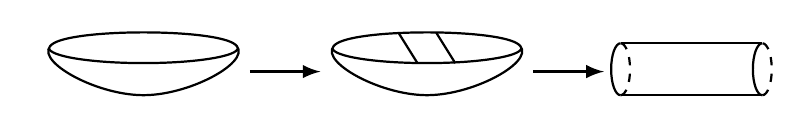
\begin{tikzpicture}[scale=1.2]
    \coordinate (p1) at (2.05,2.55);
    \coordinate (p2) at (3,2);
    \coordinate (p3) at (3.95,2.55);
    \path[draw, thick] plot [smooth cycle,tension=1] coordinates {(p1) (p2) (p3)};
    \draw[thick] (2,2.5) arc (180:360:1 and .16);
    \draw[very thick, arrow] (4, 2.25) -- (5,2.25);
    \coordinate (p1) at (5.05,2.55);
    \coordinate (p2) at (6,2);
    \coordinate (p3) at (6.95,2.55);
    \path[draw, thick] plot [smooth cycle,tension=1] coordinates {(p1) (p2) (p3)};
    \draw[thick] (5,2.5) arc (180:360:1 and .16);
    \draw[thick] (5.7,2.66) -- ++(0.2,-.32);
    \draw[thick] (6.1,2.66) -- ++(0.2,-.32);
    \draw[very thick, arrow] (7, 2.25) -- (8,2.25);
    \draw[thick] (8.05,2.55) -- ++(1.5,0);
    \draw[thick] (8.05,2) -- ++(1.5,0);
    \draw[thick] (8.05,2) arc (270:90:.1 and .275);
    \draw[thick,dashed] (8.05,2) arc (-90:90:.1 and .275);
    \draw[thick] (9.55,2) arc (270:90:.1 and .275);
    \draw[thick,dashed] (9.55,2) arc (-90:90:.1 and .275);
\end{tikzpicture}\\
    \textsc{Figure 5} – \textit{Espace obtenu après la première valeur critique (à gauche) et après la seconde (à droite)}
\end{center}


\newpage

\nocite{*}
\bibliographystyle{plain}
\bibliography{biblio}



\end{document}
